\section*{CHAPTER 1. INTRODUCTION}
\addcontentsline{toc}{section}{\numberline{}CHAPTER 1. INTRODUCTION}

\setcounter{section}{1}
\setcounter{subsection}{0}
\setcounter{figure}{0}
\setcounter{table}{0}
\setcounter{equation}{0}

%============================================================%
\subsection{Background}

Modern wireless communication systems require high data rate, efficient
spectrum utilization, and reliable transmission under multipath fading
conditions. Orthogonal Frequency Division Multiplexing (OFDM) has become
one of the most widely adopted multicarrier transmission techniques due to
its robustness against frequency-selective channels and its simple
frequency-domain equalization process.

Despite these advantages, OFDM suffers from high Peak-to-Average Power
Ratio (PAPR), which causes nonlinear distortion when practical power
amplifiers operate near saturation. This issue is particularly critical in
mobile uplink transmission, where battery efficiency and transmitter power
consumption are important design constraints.

Single-Carrier Frequency Division Multiple Access (SC-FDMA) was introduced
to address this limitation by combining single-carrier signal properties
with frequency-domain equalization. For this reason, SC-FDMA was selected
for Long Term Evolution (LTE) uplink systems.

%============================================================%
\subsection{Problem Statement}

Although OFDM provides excellent spectral efficiency and implementation
simplicity, its large signal peaks reduce amplifier efficiency and may
increase out-of-band emissions. Therefore, it is necessary to investigate
alternative transmission schemes that preserve OFDM benefits while reducing
PAPR.

SC-FDMA is considered one of the most practical solutions. A systematic
comparison between OFDM and SC-FDMA helps clarify their advantages,
limitations, and appropriate deployment scenarios.

%============================================================%
\subsection{Objectives}

The objectives of this report are:

\begin{itemize}
    \item To review the operating principles of OFDM and SC-FDMA.
    \item To compare the two systems in terms of Bit Error Rate (BER).
    \item To evaluate and compare Peak-to-Average Power Ratio (PAPR).
    \item To discuss the practical reason SC-FDMA is preferred in uplink systems.
\end{itemize}

%============================================================%
\subsection{Report Structure}

This report is organized into four chapters:

\begin{itemize}
    \item Chapter 1 introduces the research motivation and objectives.
    \item Chapter 2 presents the theoretical background of OFDM and SC-FDMA.
    \item Chapter 3 describes simulation methodology and performance results.
    \item Chapter 4 summarizes the main conclusions.
\end{itemize}

%============================================================%
\subsection{Example Table Format}

\begin{table}[H]
    \centering
    \caption{Experiment results}
    \begin{tabularx}{0.85\textwidth}{
        | >{\centering}y
        | >{\centering\arraybackslash}a
        | >{\centering\arraybackslash}a
        | >{\centering\arraybackslash}y|
    }
    \hline
    \bfseries No.
    & \bfseries Voltage (mV)
    & \bfseries Reference (mV)
    & \bfseries Error (\%) \\
    \hline
    1 &   &   &   \\ \hline
    2 &   &   &   \\ \hline
    3 &   &   &   \\ \hline
    ... &   &   &   \\ \hline
    \end{tabularx}
    \label{tab:example1}
\end{table}

%============================================================%
\subsection{Example Equation Format}

\begin{equation}
\label{eq:example1}
F(x)=\int_b^a \frac{1}{3}x^3
\end{equation}

Equation \ref{eq:example1} is an example of equation formatting in LaTeX.

%============================================================%
\subsection{Example Figure Format}

\begin{figure}[H]
    \centering
    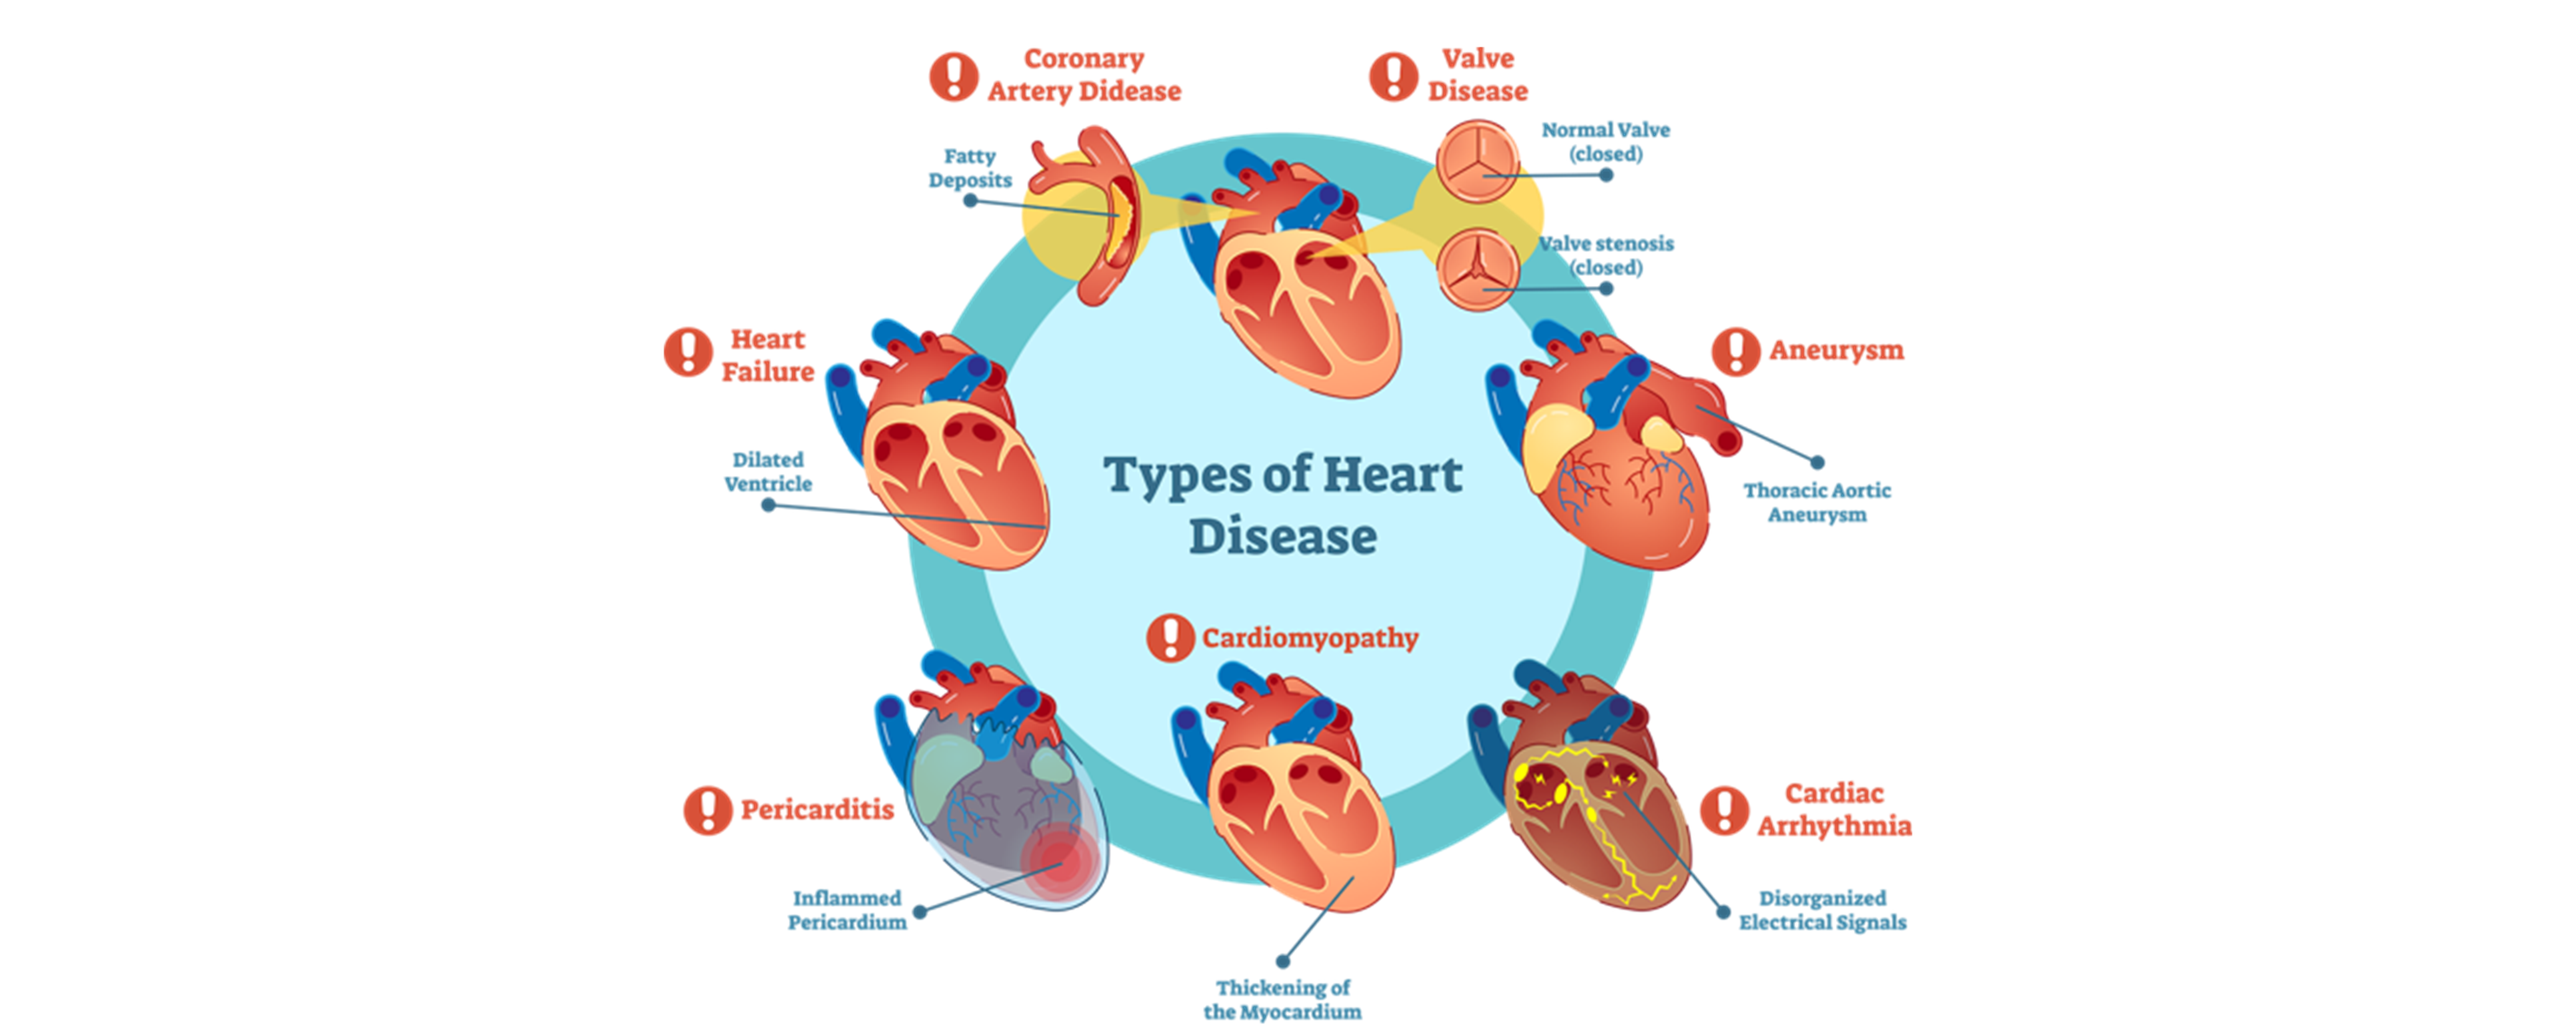
\includegraphics[width=0.95\textwidth]{Figures/Fig0.png}
    \caption{\bfseries Example figure format}
    \label{fig:example1}
\end{figure}

Figure \ref{fig:example1} illustrates an example image placeholder for later replacement.